% Default Compiler: txs:///xelatex | txs:///bibtex
% Default Bibliography Tool: BibTex

\documentclass[12pt,onecolumn,a4paper]{article}
\usepackage{listings}
\usepackage{epsfig,graphicx,subfigure,amsthm,amsmath}
\usepackage{caption}
%\usepackage{color}
\usepackage[table, svgnames, usenames,dvipsnames]{xcolor} \usepackage{array}
\usepackage{etoolbox}
\usepackage{cellspace}
\usepackage{float}
\usepackage{hhline}
\usepackage[linktocpage=true,colorlinks,citecolor=blue,pagebackref=true]{hyperref}
\usepackage[top=30mm, bottom=30mm, left=30mm, right=30mm]{geometry}
%\usepackage[T1]{fontenc}
\usepackage[utf8]{inputenc}
\usepackage{fontspec}
\setmainfont{Doulos SIL}
\usepackage{authblk}
\usepackage{polyglossia}
\setotherlanguage{english}
\setotherlanguage{persian}
\usepackage[nonamebreak]{natbib}
\usepackage{xepersian}
\settextfont[Scale=1.2]{IRLotus}
\defpersianfont\mfo[Scale=1.2]{IRLotus}
\setlatintextfont[Scale=1]{Doulos SIL}

\setcounter{Maxaffil}{0}
\renewcommand\Authands{ و }
\renewcommand\Authand{ و }
\renewcommand\Affilfont{\itshape\small}
\providecommand{\keywords}[1]{\textbf{\textit{کلیدواژه‌ها:}} #1}

\setlength\cellspacetoplimit{4pt}
\setlength\cellspacebottomlimit{4pt}
\colorlet{headercolour}{DarkSeaGreen!40}

\DefaultMathsDigits

\definecolor{customblue}{RGB}{235,241,245}
\definecolor{light-gray}{gray}{0.95}
\lstdefinestyle{C++Style}{%
backgroundcolor=\color{customblue},
breaklines=true,
basicstyle=\footnotesize\ttfamily,
keywordstyle=\color{blue},
commentstyle=\color{OliveGreen}\textit,
stringstyle=\color{red},
numbers=left,
numberstyle={\tiny\lr},
showspaces = false,
showstringspaces = false,
tabsize = 2,
frame=single,
xleftmargin=5pt,
xrightmargin=3pt,
language = C++,
aboveskip = 20pt,
rulecolor=\color{black},
captiondirection=RTL,
}

\lstnewenvironment{C++Code}[1][]
{%
\lstset{style=C++Style, #1}%
}{%
}

\def\lstlistingname{شبه‌کد}

\begin{document}
    \title{مقایسه ساخت آوایی گونهٔ رسمی و محاوره‌ای زبان فارسی\footnote{فصلنامه پازند، سال 8، شماره 30، پاییز 1391، صص 118-107}}
    \author[1]{وحید مواجی}
    \author[2]{محرم اسلامی}
    \affil[1]{دانشگاه صنعتی شریف}
    \affil[2]{دانشگاه زنجان}
    \date{15 آذر 1391}
    \maketitle

    \begin{abstract}
        گونهٔ رسمی و گونهٔ محاوره‌ای زبان‌ها غالباً با هم تفاوت‌ دارند و این تفاوت در همهٔ سطح‌های زبانی دیده می‌شود. میزان تفاوت بین گونهٔ رسمی و گونهٔ محاوره‌ای، که گاهی از آنها با عنوان تفاوت گفتار و نوشتار یاد می‌شود، از زبانی به زبان متفاوت است. زبان فارسی از جملهٔ زبان‌های است که در آن تفاوت گونهٔ رسمی و گونهٔ محاوره‌ای بسیار زیاد است. در این تحقیق تفاوت‌ها آوایی و به عبارتی فرایندهای آوایی را بررسی می‌کنیم که در زبان فارسی در تبدیل گونهٔ رسمی به گونهٔ محاوره‌ای رخ می‌دهد. مبنای پژوهش حاضر دادگان گفتاری فارسدات تلفنی زبان فارسی \Latincite{bijankhan_2003} است که در آن گفتار پیوسته
        \footnote{\lr{continuous‬‬}-\rl{گفتار پیوسته در علم گفتار به گفتار ضبط شده اطلاق می‌شود که به دو روش خوانده‌شده از روی متن و یا مستقیماً به‌دست می‌آید.}}
        در دو سطح
        \footnote{در طراحی فارسدات گفتار پیوسته در دو سطح مجزای واجی و آوایی برچسب خورده است.}
        واجی \LTRfootnote{\lr{‫‪phonemic‬‬}} و آوایی \LTRfootnote{‫‪\lr{phonetic‬}‬} در قالب دو زنجیرهٔ مستقل برچسب خورده است. هم‌گذاری این دو رشته از داده‌ها روشن می‌سازد که در مقایسهٔ این دو گونهٔ زبانی کدام فرایندهای آوایی در تبدیل زنجیرهٔ واجی به زنجیرهٔ آوایی دخیل بودند. در انطباق دو رشتهٔ واجی و آوایی از الگوریتم لونشتاین \LTRfootnote{\lr{‫‪Levenshtein‬‬}} استفاده کرده‌ایم که مناسب و رایج در انطباق تقریبی رشته‌های متفاوت جهت یافتن فاصلهٔ بین آنها است. در نتیجه تفاوت دو رشتهٔ واجی و آوایی به‌صورت آماری به‌دست آمد. از نتایج این پژوهش می‌توان به لحاظ نظری در توصیف‌های زبان‌شناختی از نظام آوایی زبان فارسی، تهیهٔ منابع محاوره‌ای زبانی فارسی و آموزش زبان فارسی به‌خصوص به غیرفارسی‌زبان‌ها سود جست. از سوی دیگر در فناوری‌های گفتار مانند بازشناسی و بازسازی گفتار، استخراج اطلاعات از متن‌های محاوره‌ای، تبدیل متن به زنجیرهٔ واجی گونهٔ محاوره‌ای زبان فارسی و امکان تبدیل آن به گونهٔ رسمی می‌توان از نتایج این تحقیق استفاده کرد.
        \par
        \keywords{ساخت آوایی، گونهٔ رسمی، گونهٔ محاوره‌ای، الگوریتم لونشتاین، فارسدات تلفنی فارسی}
    \end{abstract}

    \section{مقدمه}
    گونه‌های رسمی و محاوره‌ای زبان فارسی در تمام سطح‌های زبان تفاوت‌های زیادی با هم دارند که این امر در مقایسه با برخی زبان‌ها بسیار چشمگیر است. در همهٔ زبان‌ها بین گونه‌های رسمی و محاوره‌ای تفاوت‌های هست و در زبان‌های که مسبوق به داشتن نظام نوشتاری دیرینه هستند، این تفاوت بیشتر به چشم می‌خورد. بنابراین زبانی که زبان علم و ادب باشد، که طبیعتاً دارای خط نیز هستند، بین گونه‌های رسمی و محاوره‌ای آن فاصله بیشتر خواهد بود. از دلایل این فاصله می‌توان به محافظه‌کارانه عمل کردن خط در انعکاس تغییرات زبان اشاره کرد که نهادهای مانند فرهنگستان زبان عامدانه در قالب یک برنامه‌ریزی زبانی متولی انجام تغییرات در خط می‌شوند. دلیل دیگر شاید این باشد که در محیط‌های علمی افراد تحصیل‌کرده کمتر حاضر می‌شوند خلاف سنت نوشتاری زبان بنویسند. این موضوع باعث می‌شود به مرور زمان گونه‌های رسمی و محاوره‌ای مثلاً از حیث نظام آوایی فاصله بگیرند وضعیتی که در زبان فارسی شاهد هستیم.
    \par
    در این پژوهش کوشیده‌ایم تفاوت‌های آوایی گونه‌های رسمی و محاوره‌ای زبان فارسی را به‌صورت آماری با استفاده از پیکرهٔ زبانی فارسدات تلفنی \Latincite{bijankhan_2003} استخراج و دسته‌بندی بکنیم. در فارسدات تلفنی گفتار پیوسته در دو سطح واجی و آوایی برچسب خورده‌اند که مقایسهٔ زنجیره نشان می‌دهد که گفتار رسمی و محاوره‌ای زبان چه تفاوت‌های آوایی با هم دارند. هم‌گذاری خوکار زنجیره‌های واجی و آوایی امر دشواری است، چراکه تحولات آوایی در همهٔ جایگاه‌های صدایی کلمه رخ می‌دهد. اینکه کدام واحد صدایی به کدام واحد صدایی تبدیل شده و کدام واحد صدایی حذف یا درج شده در بررسی خودکار دشواری‌های را ایجاد می‌کند. تغییرات آوایی را می‌توان به چند دسته یا عمل تقسیم کرد:
    \par\noindent
    الف. عمل درج: مثلاً \lr{/mehrban/} با درج \lr{/a/} به \lr{/mehraban/} تبدیل می‌شود. \\
    ب. عمل حذف: مثلاً \lr{/dast/} با حذف همخوان پایانی به \lr{/das/} تبدیل می‌شود. \\
    ج. عمل جانشینی: مثلاً \lr{/?ejtemâ?/} با جانشینی \lr{/š/} به جای \lr{/j/} و حذف همزهٔ پایانی به \lr{/?eštemâ/} تبدیل می‌شود.
    \par
    چناچه در ج) می‌بینیم چندین عمل می‌توانند هم‌زمان روی یک رشته اِعمال شوند. مثلاً در مثال ج) عمل حذف، همزۀ پایانی کلمه را نیز حذف کرده است. عمل‌های ذکرشده منحصر به یک نویسۀ واحد نمی‌باشند و می‌توانند روی گروهی از نویسه‌ها اِعمال شوند، مثلاً می‌گویند تبدیل می‌شود به می‌گن که در آن گروه رشتهٔ آوایی \lr{/-uyand/} کلاً با گروه \lr{/-an/} جانشین شده است.
    \par
    برای این که فرایندهای آوایی عمل کنند، باید بافتِ آوایی را هم در نظر داشته باشیم که در این مقاله، ما از واج قبلی و واج بعدی به عنوان بافت آوایی استفاده کرده‌ایم. پیکرهٔ فارسدات تلفنی حاوی صورت واجی و آوایی کلماتی است که از ضبط صدای افراد پشت تلفن بدست آمده است. اگر صورت‌های واجی و آوایی را به‌صورت مجموعه یا رشته‌هایی از نویسه‌ها در نظر بگیریم، مسأله به تعیین میزان فاصلۀ دو رشته کاهش می‌یابد. یعنی هر چه فاصلۀ دو رشته کمتر باشد مشابهت بیشتری به هم دارند. بنابراین تغییر واجی از روی فاصلۀ کمینۀ بین دو رشته بدست خواهد آمد.
    \par
    الگوریتم‌های مختلفی برای سنجش فاصلۀ دو رشته وجود دارد که ما در این پژوهش از الگوریتم لونشتاین \Latincite{levenshtein_1966} استفاده کرده‌ایم. البته این الگوریتم فاصلۀ کمینۀ دو رشته را محاسبه می‌کند، ولی مراحل اِعمال عمل‌های مختلف (درج، حذف، جانشینی) را نمی‌دهد. لذا با تغییری که در این الگوریتم داده شد، مراحل اِعمال عمل‌های واجی هم بدست آمد.
    در این مقاله گونهٔ گفتاری معیار
    \footnote{درطراحی فارسدات تلفنی پیش‌بینی شده بود که بخش بزرگی از داده‌ها از گفتار گویشورانی اخذ شود که به گونهٔ رسمی زبان فارسی (معیار) سخن می‌گویند. در این پژوهش فقط به بررسی فرایندهای آوایی در این‌گونهٔ زبانی پرداخته‌ایم.}
    زبان فارسی از فارسدات تلفنی مدنظر است.

    \section{معیارهای مشابهت}
    برای ارزیابی میزان شباهت یا عدم شباهت (فاصله) دو رشته نسبت به یکدیگر از معیارهای مشابهت رشته‌ای استفاده می‌شود. معیار مشابهت یک عدد اعشاری است که درجه مشابهت دو رشته از نویسه‌ها را مشخص می‌سازد. مثلاً فاصلۀ بین دو رشتۀ رایانه و پایانه کمتر از فاصلۀ بین دو رشتۀ رایانه و یارانه است.
    \par
    از معیارهای مشابهت در زمینه‌های مختلفی منجمله تطابق تقریبی رشته‌ها \Latincite{navarro_2001}، مقایسه \Latincite{stoilos_2005} و جستجوی فازی رشته‌ها \Latincite{jin_2005} استفاده می‌شود. یکی از پرکاربردترین زمینه‌های آن، خطایاب‌های املایی \Latincite{li_2008} است، بدین صورت که متنی به عنوان ورودی به خطایاب داده می‌شود و خطایاب باید کلمات اشتباه را با نزدیک‌ترین کلمات (کلماتی با بیشترین میزان مشابهت و کمترین فاصله) جایگزین سازد. در ادامه پرکاربردترین معیارهای فاصلۀ دو رشته معرفی شده‌اند.

    \subsection{فاصلۀ لونشتاین\protect\LTRfootnote{\lr{Levenshtein distance}}}
    فاصلۀ لونشتاین \Latincite{levenshtein_1966} به صورت حداقل میزان تغییرات مورد نیاز برای رشتۀ S به رشتۀ T تعریف می‌شود که عملیات مجاز در آن عبارتند از: درج، حذف یا جانشینی یک نویسۀ واحد. برای مثال فاصلۀ لونشتاین دو رشتۀ apple و orange با یک ماتریس ساده در جدول \ref{table:1} محاسبه شده است. فاصلۀ این دو رشته برابر 5 است که در قسمت پایین و سمت راست ماتریس نشان داده شده است. این فاصله بدین معناست که رشتۀ apple را با درج \lr{o}، جانشینی \lr{r} به جای \lr{a}، \lr{a} به جای \lr{p}، \lr{n} به جای \lr{p} و \lr{g} به جای \lr{l} به رشتۀ orange تبدیل می‌شود. یک عملیات درج و چهار عملیات جانشینی داریم که مجموعاً برابر 5 می‌شود.


    \begin{table}[H]
        \caption{مثالی از فاصلۀ لونشتاین}
        \label{table:1}
        \centering\setLTR
        \begin{tabular}{c|ccccccc|}
            \multicolumn{1}{c}{} & \multicolumn{1}{c}{} & \cellcolor{blue!25}A & \cellcolor{blue!25}P & \cellcolor{blue!25}P & \cellcolor{blue!25}L & \cellcolor{blue!25}E \tabularnewline \hhline{~|*{6}{-}}
            & 0 & 1 & 2 & 3 & 4 & 5  \tabularnewline
            \cellcolor{blue!25}O & 1 & 1 & 2 & 3 & 4 & 5   \tabularnewline
            \cellcolor{blue!25}R & 2 & 2 & 2 & 3 & 4 & 5   \tabularnewline
            \cellcolor{blue!25}A & 3 & 2 & 3 & 3 & 4 & 5   \tabularnewline
            \cellcolor{blue!25}N & 4 & 3 & 3 & 4 & 4 & 5   \tabularnewline
            \cellcolor{blue!25}G & 5 & 4 & 4 & 4 & 5 & 5   \tabularnewline
            \cellcolor{blue!25}E & 6 & 5 & 5 & 5 & 5 & 5   \tabularnewline
        \end{tabular}
        \setRTL
    \end{table}

    \par
    مراحل ساخته شدن ماتریس شکل 1 به شرح ذیل است:
    \begin{enumerate}
        \item ماتریس $d$ با $M$ سطر و $N$ ستون ساخته می‌شود.
        \item به سطر اول مقادیر از $0$ تا $M$ و به ستون اول مقادیر از $0$ تا $N$ اختصاص داده می‌شود.
        \item هر نویسه‌ای از $S$ ($i$ از $1$ تا $M$)  و هر نویسه‌ای از $T$ ($j$ از $1$ تا $N$) را بررسی می‌کنیم.
        \item اگر $S[i]$ با $T[j]$ برابر بود، هزینه برابر $0$ و در غیر این صورت برابر $1$ است.
        \item مقدار عنصر $d[i, j]$ ماتریس برابر کمینه مقادیر زیر است:
        \begin{enumerate}
            \item عنصر بالایی بعلاوۀ یک: $d[i-1, j]+1$
            \item عنصر سمت چپ بعلاوۀ یک: $d[i, j-1]+1$
            \item عنصر بالا و سمت چپ بعلاوۀ هزینه: $d[i-1, j-1]+cost$
        \end{enumerate}
        \item بعد از این که تکرار مراحل 3، 4 و 5 به پایان رسید، مقدار فاصله در عنصر $d[N,M]$ قرار دارد.
    \end{enumerate}

    \par
    شبه‌کد فاصلۀ لونشتاین در شبه‌کد \ref{listing:1} آمده است.

    \begin{LTR}
        %@formatter:off
        \begin{lstlisting}[style=C++Style,caption=\rl{فاصلۀ لونشتاین}, label={listing:1}]
        int LevenshteinDistance(char S[1..M], char T[1..N]){
            declare int d[0..M, 0..N]
            for i from 0 to M
                d[i,0] := i //the distance of any first string to an empty second string
            for j from 0 to N
                d[0, j] := j //the distance of any second string to an empty first string
            for j from 1 to N
            {
                for i from 1 to M
                {
                    if S[i] = T[j] then
                        d[i, j] := d[i-1, j-1] //no operation required
                    else d[i, j] := minimum(d[i-1, j] + 1, //a deletion
                                d[i, j-1] + 1, //an insertion
                                d[i-1, j-1] + 1) //a substitution
                }
            }
            return d[M, N]
        }
        \end{lstlisting}
        %@formatter:on
    \end{LTR}

    \subsection{فاصلۀ همینگ\protect\LTRfootnote{\lr{Hamming distance}}}
    فاصلۀ همینگ \Latincite{hamming_1950} فقط عملیات جانشینی را برای تبدیل $S$ به $T$ مجاز می‌شمارد. بنابراین طول $S$ و $T$ باید برابر باشد. از این الگوریتم بیشتر برای تشخیص و تصحیح خطا برای دو رشته با طول مساوی استفاده می‌شود. پیاده‌سازی فاصلۀ همینگ در شبه‌کد \ref{listing:2} آمده است. این الگوریتم، دو رشتۀ $S$ و $T$ را به عنوان ورودی گرفته و فاصلۀ همینگ آنها را برمی‌گرداند.

    \begin{LTR}
        %@formatter:off
        \begin{lstlisting}[style=C++Style,caption=\rl{فاصلۀ همینگ}, label={listing:2}]
        int HammingDistance(S[1..M], T[1..N])
        {
            If M !=N then return -1
            declare int HammingDistance=0
            for i from 1 to M{
                if S[i] != T[i] then HammingDistance++
            }
            return HammingDistance
        }
        \end{lstlisting}
        %@formatter:on
    \end{LTR}

    \subsection{فاصلۀ دامرو-لونشتاین\protect\LTRfootnote{\lr{Damerau-Levenshtein distance}}}
    فاصلۀ دامرو-لونشتاین \Latincite{damerau_1964} مشابه فاصلۀ لونشتاین است. تنها فرق آن این است که فاصلۀ دامرو-لونشتاین یک عملیات دیگر را مجاز می‌شمارد: ترانهش\LTRfootnote{\lr{Transposition}}  دو نویسۀ مجاور. شبه‌کد محاسبۀ فاصلۀ دامرو-لونشتاین در شبه‌کد \ref{listing:3} آمده است.

    \begin{LTR}
        %@formatter:off
        \begin{lstlisting}[style=C++Style,caption=\rl{فاصلۀ دامرو-لونشتاین}, label={listing:3}]
        int DamerauLevenshteinDistance(char S[1..M], char T[1..N])
        {
            declare int d[0..M, 0..N]
            declare int i, j, cost
            for i from 0 to M
                d[i,0] := i //the distance of any first string to an empty second string
            for j from 0 to N
                d[0, j] := j //the distance of any second string to an empty first string
            for i from 1 to M
            {
                for j from 1 to N{
                if S[i] = T[j] then cost := 0
                        else cost := 1
                    d[i, j] := minimum(d[i-1, j] + 1, //a deletion
                                d[i, j-1] + 1, //an insertion
                                d[i-1, j-1] + 1) //a substitution
                if(i > 1 and j > 1 and S[i] = T[j-1] and S[i-1] = M[j]) then
                    d[i, j] := minimum(
                                d[i, j],
                                d[i-2, j-2] + cost) // transposition
                }
            }
            return d[M, N]
        }
        \end{lstlisting}
        %@formatter:on
    \end{LTR}

    \par
    در این مقاله از روش فاصلۀ لونشتاین استفاده کرده‌ایم و در آن تغییراتی داده‌ایم که جابجایی یک گروه با یک گروه دیگر را و اینکه چه مجموعه نویسه‌ای به چه مجموعه نویسه‌ای تبدیل شده‌ است را نیز بدست می‌آوریم. در الگوریتم استاندارد لونشتاین، تغییرات یک نویسه درنظرگرفته می‌شود و درنهایت نیز خروجی الگوریتم برابر فقط حداقل مراحل تغییرات است که در خانه پایین و راست ماتریس موردنظر قرار دارد.

    \section{روش کار}
    در پیکرهٔ زبانی این تحقیق (فارس‌دات تلفنی) مجموعه‌ای شامل 282553 ردیف داده قرار دارد. اطلاعات موجود در هر سطر این پیکره شامل موارد زیر است:

    \begin{itemize}
        \item صورت واجی (Phonemic) مانند hastid
        \item صورت آوایی \footnote{از آنجایی که این تفاوت‌ها حاصل اعمال فرایندهای آوایی در یک زبان واحد است، لذا به این صورت‌ها که اشتقاق روساخت از زیرساخت به حساب می‌آیند، صورت واجی و آوایی اطلاق می‌شود.} (Phonetic) مانند hastin
        \item صورت نوشتاری فارسی مانند هستید
        \item زمان شروع و زمان پایان گفتار.
    \end{itemize}

    \par
    برای کار مورد نظر ما، همهٔ سطرهای این پیکره دارای ارزش اطلاعاتی نبودند، چرا که برخی اطلاعات مانند مکث، تپق، خنده، سرفه و ... نیز در این پیکره ذخیره شده است. لذا در مرحله اول کار، پیکره از این گونه اطلاعات پالایش شد و 219586 سطر از اطلاعات باقی ماند. از این مقدار نیز، مقادیر زیادی دارای صورت واجی و آوایی یکسانی بودند که این گونه اطلاعات نیز پالایش شد و در نتیجه 16950 سطر دارای زنجیره‌های واجی و آوایی متفاوت باقی ماند. سپس الگوریتم تفاوت‌یابی رشته‌های که در مرحله قبل توضیح داده شد روی این تعداد داده اعمال گردید که تعداد 13527 تغییر بدست آمد. البته این میزان تغییرات دارای تکرار بود و در بررسی دقیقتر، تعداد تغییرات برابر 2793 نوع بود. ما برای بررسی بسامد تغییرات آوایی، تغییرات با تکرار را در نظر گرفتیم تا به یک تحلیل آماری از میزان تغییرات در آواها هنگام صحبت روزمره برسیم.

    \section{نتایج به دست آمده}
    تعداد زیادی از این تغییرات دارای بسامد کمی (حتی یک بار) بودند و تعداد کمی از این تغییرات دارای بسامد زیاد. همانطور که در نمودارهای زیر مشاهده می‌کنیم، درصد کمی از تغییرات، بیشترین میزان توزیع بسامدی را اشغال کرده‌اند، یعنی تقریباً 30 تغییر اول بیشترین بسامد را دارند و مابقی تغییرات دارای بسامد و احتمال وقوع کمتری می‌باشند. نمودار توزیع فراوانی 30 تغییر اول در شکل \ref{fig:1} و نمودار توزیع فراوانی 90 تغییر اول در شکل \ref{fig:2} آمده است. جدول \ref{table:2} جدول توزیع فراوانی 30 تغییر اول را با جزئیات بیشتری مشخص می‌سازد. مثالی از تغییرات پربسامد به شرح زیر می‌باشد:
    \footnote{علامت \$ در شکل‌ها و جداول، پیش یا پس از تبدیل آوایی، بیانگر جایگاه فرایند آوایی در اول یا آخر کلمه است.}
    \footnote{در فارسدات تلفنی /k/ صورت زیرساختی قلمداد شده است که در روساخت به دو صورت [k] پسکامی و [c] پیشکامی بازنمایی می‌شود.}

    \begin{LTR}
        \begin{itemize}
            \item \lr{šân} $\rightarrow$ \lr{šun}
            \item \lr{nd} $\rightarrow$ \lr{n}
            \item \lr{mân} $\rightarrow$ \lr{mun}
            \item \lr{?e} $\rightarrow$ \lr{e}
            \item \lr{?a} $\rightarrow$ \lr{a}
            \item \lr{rh} $\rightarrow$ \lr{r}
            \item \lr{ka} $\rightarrow$ \lr{ca}
            \item \lr{tân} $\rightarrow$ \lr{tun}
            \item \lr{ihâ} $\rightarrow$ \lr{iyâ}
            \item \lr{âyaš} $\rightarrow$ \lr{âš}
            \item \lr{?â} $\rightarrow$ \lr{â}
            \item \lr{nhâ} $\rightarrow$ \lr{nâ}
        \end{itemize}
    \end{LTR}

    \begin{table}[H]
        \caption{نمودار توزیع فراوانی 30 تغییر اول}
        \label{table:2}
        \centering\setLTR
        \begin{tabular}{|c|c|c|c|c|c|c|c|c|}
            \hline
            \cellcolor{blue!25}ردیف & \cellcolor{blue!25}\rl{تبدیل آوایی} & تعداد\cellcolor{blue!25} & \cellcolor{blue!25}ردیف & \cellcolor{blue!25}\rl{تبدیل آوایی} & تعداد\cellcolor{blue!25} & \cellcolor{blue!25}ردیف & \cellcolor{blue!25}\rl{تبدیل آوایی} & \cellcolor{blue!25}تعداد    \tabularnewline \hline

            \cellcolor{blue!25}1 & {\lr{šân}  $\rightarrow$ \lr{šun}}  & 472 & \cellcolor{blue!25}11 & {\lr{âyaš} $\rightarrow$ \lr{âš}}   & 131 & \cellcolor{blue!25}21 & {\lr{id\$} $\rightarrow$ \lr{in\$}} & 89 \tabularnewline
            \cellcolor{blue!25}2 & {\lr{he}   $\rightarrow$ \lr{hye}}  & 469 & \cellcolor{blue!25}12 & {\lr{\$?â} $\rightarrow$ \lr{\$â}}  & 131 & \cellcolor{blue!25}22 & {\lr{dhâ}  $\rightarrow$ \lr{dâ}}   & 85 \tabularnewline
            \cellcolor{blue!25}3 & {\lr{nd\$} $\rightarrow$ \lr{n\$}}  & 354 & \cellcolor{blue!25}13 & {\lr{nhâ}  $\rightarrow$ \lr{nâ}}   & 128 & \cellcolor{blue!25}23 & {\lr{re}   $\rightarrow$ \lr{rye}}  & 68 \tabularnewline
            \cellcolor{blue!25}4 & {\lr{mân}  $\rightarrow$ \lr{mun}}  & 323 & \cellcolor{blue!25}14 & {\lr{egi}  $\rightarrow$ \lr{eji}}  & 126 & \cellcolor{blue!25}24 & {\lr{lhâ}  $\rightarrow$ \lr{lâ}}   & 65 \tabularnewline
            \cellcolor{blue!25}5 & {\lr{\$?e} $\rightarrow$ \lr{\$e}}  & 246 & \cellcolor{blue!25}15 & {\lr{e?i}  $\rightarrow$ \lr{ei}}   & 126 & \cellcolor{blue!25}25 & {\lr{\$ge} $\rightarrow$ \lr{\$je}} & 63 \tabularnewline
            \cellcolor{blue!25}6 & {\lr{\$?a} $\rightarrow$ \lr{\$a}}  & 203 & \cellcolor{blue!25}16 & {\lr{\$ke} $\rightarrow$ \lr{\$ce}} & 124 & \cellcolor{blue!25}26 & {\lr{dân}  $\rightarrow$ \lr{dun}}  & 60 \tabularnewline
            \cellcolor{blue!25}7 & {\lr{rhâ}  $\rightarrow$ \lr{râ}}   & 170 & \cellcolor{blue!25}17 & {\lr{xân}  $\rightarrow$ \lr{xun}}  & 113 & \cellcolor{blue!25}27 & {\lr{\$?i} $\rightarrow$ \lr{\$i}}  & 59 \tabularnewline
            \cellcolor{blue!25}8 & {\lr{\$ka} $\rightarrow$ \lr{\$ca}} & 162 & \cellcolor{blue!25}18 & {\lr{iyaš} $\rightarrow$ \lr{iš}}   & 106 & \cellcolor{blue!25}28 & {\lr{ike}  $\rightarrow$ \lr{ice}}  & 57 \tabularnewline
            \cellcolor{blue!25}9 & {\lr{tân}  $\rightarrow$ \lr{tun}}  & 154 & \cellcolor{blue!25}19 & {\lr{âyeš} $\rightarrow$ \lr{âš}}   & 105 & \cellcolor{blue!25}29 & {\lr{shâ}  $\rightarrow$ \lr{sâ}}   & 55 \tabularnewline
            \cellcolor{blue!25}10 & {\lr{ihâ}  $\rightarrow$ \lr{iyâ}}  & 154 & \cellcolor{blue!25}20 & {\lr{thâ}  $\rightarrow$ \lr{tâ}}   & 96 & \cellcolor{blue!25}30 & {\lr{ehâ}  $\rightarrow$ \lr{eâ}}   & 54 \tabularnewline \hline

        \end{tabular}
        \setRTL
    \end{table}

    \begin{figure}[H]
        \centering
        \makebox[\textwidth]{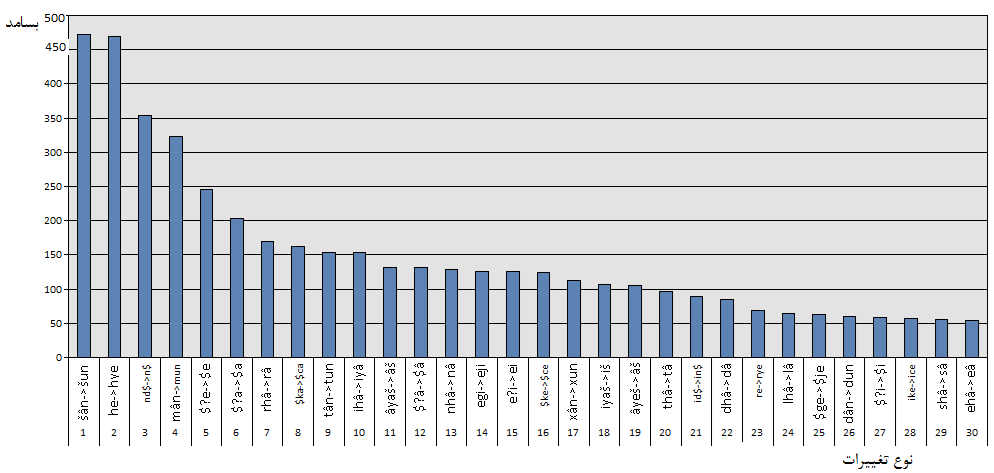
\includegraphics[width=\textwidth]{pazand5.png}}
        \caption{نمودار توزیع فراوانی 30 تغییر اول}
        \label{fig:1}
    \end{figure}

    \begin{figure}[H]
        \centering
        \makebox[\textwidth]{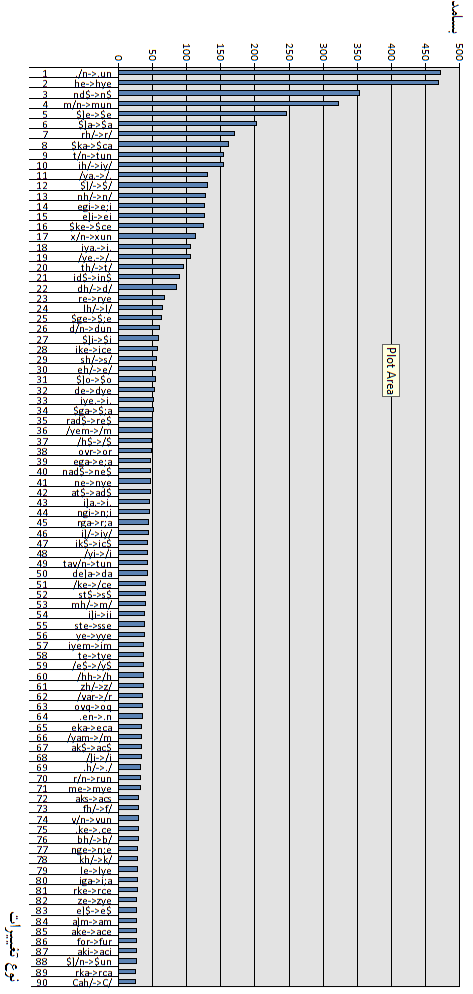
\includegraphics[width=\textwidth,height=0.9\textheight,keepaspectratio]{pazand6.png}}
        \caption{نمودار توزیع فراوانی 90 تغییر اول}
        \label{fig:2}
    \end{figure}

    \section{نتیجه‌گیری}
    در این تحقیق ساخت آوایی گونهٔ رسمی و محاوره‌ای زبان فارسی براساس پیکرهٔ زبانی فارسدات تلفنی مورد بررسی قرار گرفت و در نتیجهٔ آن نوع و بسامد تحولات آوایی در زبان فارسی در چارچوب پیکرهٔ زبانی موردنظر مشخص شد. نوع تحولات آوایی محدود به عمل‌های جانشینی، حذف و درج بود که از مقایسهٔ فاصلهٔ نویسه‌های مربوط به کلمه‌ها در دو سطح واجی و آوایی موجود در فارسدات تلفنی به‌دست می‌آمد. با انجام تغییراتی از الگوریتم لونشتاین برای مقایسهٔ خوکار عمل‌های جانشینی، حذف و درج استفاده کردیم. در ارزیابی نتیجهٔ پژوهش مشخص شد که تعداد زیادی از این تغییرات دارای بسامد کم و تعداد کمی از تغییرات دارای بسامد زیاد بودند. شکل‌های \ref{fig:1} (نیز در جدول \ref{table:2}) و \ref{fig:2} به‌ترتیب توزیع فراوانی 30 و 90 تغییر اول را با جزئیات بیشتری مشخص می‌سازند.
    \par
    از نتایج این پژوهش می‌توان به لحاظ نظری در توصیف‌های زبان‌شناختی از نظام آوایی زبان فارسی، تهیهٔ منابع محاوره‌ای زبانی فارسی و آموزش زبان فارسی به‌خصوص به غیرفارسی‌زبان‌ها سود جست. از سوی دیگر در فناوری‌های گفتار مانند بازشناسی و بازسازی گفتار، استخراج اطلاعات از متن‌های محاوره‌ای، تبدیل متن به زنجیرهٔ واجی گونهٔ محاوره‌ای زبان فارسی و امکان تبدیل آن به گونهٔ رسمی می‌توان از نتایج این تحقیق استفاده کرد.

    {\mfo
    \bibliographystyle{asa-fa}
    \bibliography{references}}

\end{document}